\documentclass[tikz, mode=buildnew]{standalone}

\begin{document}
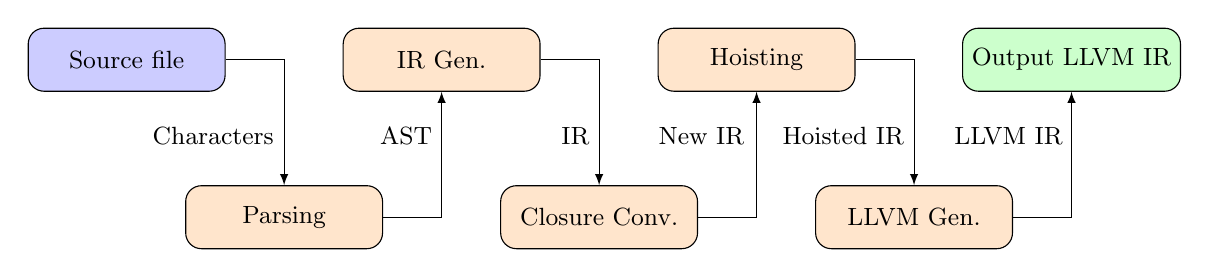
\begin{tikzpicture}[node distance=2cm, auto]
    \tikzstyle{beginend} = [draw, rectangle, rounded corners=2mm, fill=blue!20, minimum width=2.5cm, minimum height=0.8cm, font=\small]
    \tikzstyle{middle} = [draw, rectangle, rounded corners=2mm, fill=orange!20, minimum width=2.5cm, minimum height=0.8cm, font=\small]
    \tikzstyle{output} = [draw, rectangle, rounded corners=2mm, fill=green!20, minimum width=2.5cm, minimum height=0.8cm, font=\small]

    \node[beginend] (source) {Source file};
    \node[middle, right of=source, below of=source] (parser) {Parsing};
    \node[middle, right of=parser, above of=parser] (irgen) {IR Gen.};
    \node[middle, right of=irgen, below of=irgen] (closure) {Closure Conv.};
    \node[middle, right of=closure, above of=closure] (hoisting) {Hoisting};
    \node[middle, right of=hoisting, below of=hoisting] (llvmgen) {LLVM Gen.};
    \node[output, right of=llvmgen, above of=llvmgen] (output) {Output LLVM IR};

    \draw[-latex] (source) -- (source -| parser) -- node[midway, above, font=\small, xshift=-0.9cm, yshift=-0.4cm] {Characters} (parser);
    \draw[-latex] (parser) -- (parser -| irgen) -- node[midway, above, font=\small, xshift=-0.45cm, yshift=-0.00cm] {AST} (irgen);
    \draw[-latex] (irgen) -- (irgen -| closure) -- node[midway, above, font=\small, xshift=-0.3cm, yshift=-0.4cm] {IR} (closure);
    \draw[-latex] (closure) -- (closure -| hoisting) -- node[midway, above, font=\small, xshift=-0.7cm] {New IR} (hoisting);
    \draw[-latex] (hoisting) -- (hoisting -| llvmgen) -- node[midway, above, font=\small, xshift=-0.9cm, yshift=-0.4cm] {Hoisted IR} (llvmgen); % New arrow
    \draw[-latex] (llvmgen) -- (llvmgen -| output) -- node[midway, above, font=\small, xshift=-0.8cm, yshift=-0.0cm] {LLVM IR} (output);
\end{tikzpicture}
\end{document}
